
% ----------------------------------------------------------------------
%  Set the document class
% ----------------------------------------------------------------------
\documentclass[11pt,a4paper,twoside]{article}

% ----------------------------------------------------------------------
% Define external packages, language, margins, fonts and new commands
% ----------------------------------------------------------------------
%\input{preamble} 
\usepackage[utf8]{inputenc}   % <<<<< Linux
\usepackage[english]{babel} % <<<<< English
\usepackage{notoccite}
\usepackage[skip=0.5\baselineskip]{caption}
\hyphenation{GTKWave}
\usepackage{listings}
\usepackage[all]{nowidow}

%blind text
\usepackage{lipsum}

\usepackage{graphicx}
\graphicspath{{./}{../../figlib/}{../mat/}{../sim/}}
\def\FontLn{% 16 pt normal
  \usefont{T1}{phv}{m}{n}\fontsize{16pt}{16pt}\selectfont}
\def\FontLb{% 16 pt bold
  \usefont{T1}{phv}{b}{n}\fontsize{16pt}{16pt}\selectfont}
\def\FontMn{% 14 pt normal
  \usefont{T1}{phv}{m}{n}\fontsize{14pt}{14pt}\selectfont}
\def\FontMb{% 14 pt bold
  \usefont{T1}{phv}{b}{n}\fontsize{14pt}{14pt}\selectfont}
\def\FontSn{% 12 pt normal
  \usefont{T1}{phv}{m}{n}\fontsize{12pt}{12pt}\selectfont}

% Use Arial font as default
%
\renewcommand{\rmdefault}{phv}
\renewcommand{\sfdefault}{phv}
\usepackage{geometry}	
\geometry{verbose,tmargin=2.5cm,bmargin=2.5cm,lmargin=2.5cm,rmargin=2.5cm}

%\usepackage{setspace}
%\renewcommand{\baselinestretch}{1.5}

\usepackage[pdftex]{hyperref} % enhance documents that are to be
                              % output as HTML and PDF
\hypersetup{colorlinks,       % color text of links and anchors,
                              % eliminates borders around links
%            linkcolor=red,    % color for normal internal links
            linkcolor=black,  % color for normal internal links
            anchorcolor=black,% color for anchor text
%            citecolor=green,  % color for bibliographical citations
            citecolor=black,  % color for bibliographical citations
%            filecolor=magenta,% color for URLs which open local files
            filecolor=black,  % color for URLs which open local files
%            menucolor=red,    % color for Acrobat menu items
            menucolor=black,  % color for Acrobat menu items
%            pagecolor=red,    % color for links to other pages
            pagecolor=black,  % color for links to other pages
%            urlcolor=cyan,    % color for linked URLs
            urlcolor=black,   % color for linked URLs
	          bookmarks=true,         % create PDF bookmarks
	          bookmarksopen=false,    % don't expand bookmarks
	          bookmarksnumbered=true, % number bookmarks
	          pdftitle={report},
            pdfauthor={Andre C. Marta},
%            pdfsubject={Thesis Title},
%            pdfkeywords={Thesis Keywords},
            pdfstartview=FitV,
            pdfdisplaydoctitle=true}

\usepackage[numbers,sort&compress]{natbib} % <<<<< References in numbered list [1],[2],...
\usepackage{subcaption} 
\usepackage{mdframed}

%%%%%%%%%%%%%%%%%%%%%%%%%%%%%%%%%%%%%%%%%%%%%%%%%%%%%%%%%%%%%%%%%%%%%%%%
%     Begin Document                                                   %
%%%%%%%%%%%%%%%%%%%%%%%%%%%%%%%%%%%%%%%%%%%%%%%%%%%%%%%%%%%%%%%%%%%%%%%%


\begin{document}

% Set plain page style (no headers, footer with centered page number)
\pagestyle{plain}

% Set roman numbering (i,ii,...) before the start of chapters
%\pagenumbering{roman}

% ----------------------------------------------------------------------
%  Cover page
% ----------------------------------------------------------------------
%%%%%%%%%%%%%%%%%%%%%%%%%%%%%%%%%%%%%%%%%%%%%%%%%%%%%%%%%%%%%%%%%%%%%%%%
%                                                                      %
%     File: Thesis_FrontCover.tex                                      %
%     Tex Master: Thesis.tex                                           %
%                                                                      %
%     Author: Andre C. Marta                                           %
%     Last modified :  2 Jul 2015                                      %
%                                                                      %
%%%%%%%%%%%%%%%%%%%%%%%%%%%%%%%%%%%%%%%%%%%%%%%%%%%%%%%%%%%%%%%%%%%%%%%%

\thispagestyle {empty}

% IST Logo - Signature A
% parameters: bb=llx lly urx ury (bounding box), width=h_length, height=v_length, angle=angle, scale=factor, clip=true/false, draft=true/false. 
\includegraphics[bb=9.5cm 11cm 0cm 0cm,scale=0.29]{IST_A_CMYK_POS}

\begin{center}
%
% Figure (Image or plot)
\vspace{1.0cm}
% height = 50 mm
%\includegraphics[height=50mm]{Figures/Airbus_A350.jpg}

% Title, author and degree
\vspace{1cm}
{\FontLb Circuit Theory and Electronics Fundamentals} \\ % <<<<< EDIT TITLE
\vspace{1cm}
{\FontLb T1} \\
\vspace{1cm}
{\FontSn Department of Electrical and Computer Engineering, Aerospace Engineering, Técnico, University of Lisbon} \\ % <<<<< EDIT COURSE
\vspace{1cm}
{\FontSn March 24, 2021} \\ % <<<<< EDIT DATE (corresponds to date of oral examination)
%
\end{center}



% ----------------------------------------------------------------------
% Dedication page (optional)
% ----------------------------------------------------------------------
%\input{dedication} 
%\cleardoublepage

% ----------------------------------------------------------------------
%  Acknowledgments (optional)
% ----------------------------------------------------------------------
%\input{acknowledgements}
%\cleardoublepage

% ----------------------------------------------------------------------
%  Abstract (both in English and Portuguese)
% ----------------------------------------------------------------------
%\input{resumo} 
%\cleardoublepage

%\input{abstract} 

% ----------------------------------------------------------------------
%  Table of contents, list of tables, list of figures and nomenclature
% ----------------------------------------------------------------------

% Table of contents
%
\tableofcontents

% List of tables
%\addcontentsline{toc}{section}{\listtablename}
%\listoftables
%\cleardoublepage 

% List of figures
%\addcontentsline{toc}{section}{\listfigurename}
%\listoffigures
%\cleardoublepage 

% Set arabic numbering (1,2,...) after preface
%
%\setcounter{page}{1}
%\pagenumbering{arabic}

% ----------------------------------------------------------------------
%  Body
% ----------------------------------------------------------------------

\section{Introduction}
\label{sec:introduction}
\paragraph{}
\par The objective of this laboratory assignment is to study a circuit in which we have the following components: two current sources ($I_b$ and $I_d$), one of them voltage dependent ($I_b$), two voltage sources ($V_a$ and $V_c$), one of them current dependent ($V_c$) and seven resistors. 
\par The circuit is represented with resort to \textit{LibreOffice Draw} and can be viewed in figure \ref{circuit}.

\begin{figure}[H]
    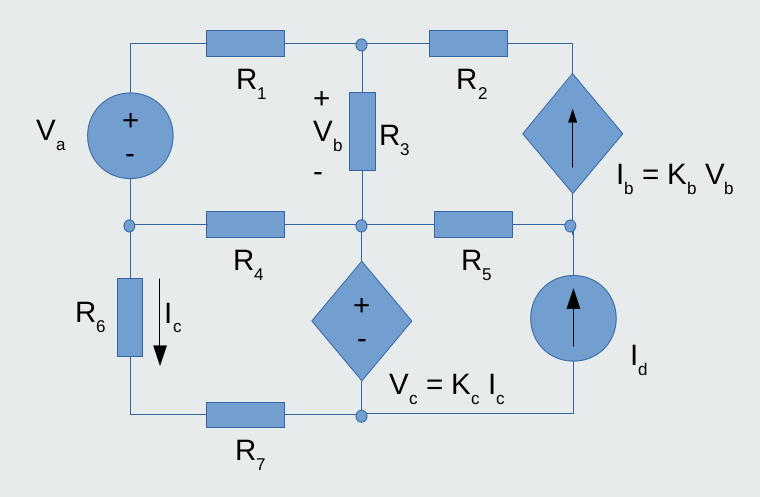
\includegraphics[width=0.8\linewidth]{Circuito.png}
    \centering
    \caption{Studied Circuit}
    \label{circuit}
\end{figure}

In Section~\ref{sec:analysis}, a theoretical analysis of the circuit is
presented. In Section~\ref{sec:simulation}, the circuit is analysed by
simulation, and the results are compared to the theoretical results obtained in
Section~\ref{sec:analysis}. The conclusions of this study are outlined in
Section~\ref{sec:conclusion}.


\section{Theoretical Analysis}
\label{sec:analysis}
\paragraph{}
\par In this section, the circuit shown in Figure \ref{circuit} is analysed
theoretically, using the two methods required, mesh and nodes. The known values can be checked in the table below.
\begin{table}[H]
    \centering
    \begin{tabular}{|c|c|}
    \hline
        $R_1$ & 1.01080769792 kOhm \\ \hline 
        $R_2$ & 2.07664633274 kOhm \\ \hline
        $R_3$ & 3.12595649013 kOhm \\ \hline
        $R_4$ & 4.18722214507 kOhm \\ \hline
        $R_5$ & 3.0841699201 kOhm  \\ \hline
        $R_6$ & 2.00179338129 kOhm \\ \hline
        $R_7$ & 1.04556537884 kOhm \\ \hline
        $V_a$ & 5.00120775651 V \\ \hline
        $I_d$ & 1.03136220214 mA \\ \hline
        $K_b$ & 7.12593545434 mS \\ \hline
        $K_c$ & 8.24048597287 kOhm \\ \hline	
    \end{tabular}
    \caption{Known Data}
    \label{data}
\end{table}
\subsection{Mesh Method}
\paragraph{}
\par A mesh is a loop that contains no other loops within it. That said, the mesh method is able to determine the current in each of the said loops, resorting to the Kirchoff Voltage Law (KVL). Having those values it is a matter of applying Ohms Law to the resistances in the mesh in order to determine the voltage in every node in the circuit, given that the values for the resistances are provided. This method is not common in automation because it is necessary to identify the different meshes, to which there may be a necessity for an outside observer.

\par Analyzing our circuit in particular, we can identify four meshes, to which we wrote the equations, stipulating a current flow for each mesh, as shown in figure \ref{mesh}. 

\begin{figure}[H]
    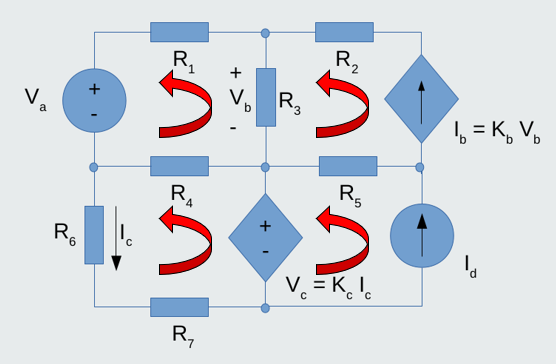
\includegraphics[width=0.5\linewidth]{Mesh.png}
    \centering
    \caption{Mesh Method applied to the circuit}
    \label{mesh}
\end{figure}

\par After simplyfying the mesh method, the system \ref{system mesh} was obtained as follows
$$
\begin{cases} 
	R_{1}I_{a}+R_{3}(I_{a}-I_{b})+R_{4}(I_{a}-I_{c}) = V_a \\ 
	R_{3}(I_{a}-I_{b})+\frac{I_{b}}{K_{b}} = 0 \\
	R_{4}(I_{a}-I_{c})-R_{6}I_{c}-R_{7}I_{c}+K_{c}I_{c} = 0 
\label{system mesh}
\end{cases}
$$


\par It was then morphed into the system below \ref{matrix} and solved with the aid of \textit{Octave}. 

\begin{equation}
	\begin{bmatrix}
		R_1+R_3+R_4 & -R_3 & -R_4 \\
		R_3 & -R_3+\frac{1}{K_b} & 0 \\
		R_4 & 0 & K_c-R_4-R_6-R_7 \\
	\end{bmatrix}
	\begin{bmatrix}
		I_a     \\
		I_b     \\
		I_c \\
	\end{bmatrix}
    =
	\begin{bmatrix}
		V_a     \\
		0     \\
		0  \\
	\end{bmatrix}
	\label{matrix}
\end{equation}

\par It was possible, after the said, to obtain the values for the voltage and current sources, as can be verified in the following table \ref{mesh}, with the current measured in mA and the voltage in V. 

\begin{table}[H]
  \centering
  \begin{tabular}{|c|c|}
    \hline    
    {\bf Name} & {\bf Value [mA]} \\ \hline
    $I_a$ & 2.224637e-01 \\ \hline 
$I_b$ & 2.329201e-01 \\ \hline 
$I_c$ & -9.260366e-01 \\ \hline 
$I_d$ & 1.031362e+00 \\ \hline 

  \end{tabular}
  \caption{Mesh method results.}
  \label{mesh}
\end{table}
\newpage
\subsection{Node Method}
\paragraph{}
\par The most crucial part in this method is to properly identify all the nodes in a circuit, which are the regions that connect two or more elements of a circuit. Then, with the aid of a system of equations provided by the Kirchoff Current Law (KCL) in the nodes unrelated to voltage sources and some extra equalities, it is possible to determine the voltage in every node. Due to the fact that we can only use KCL like previously explained, the aforementioned extra equalities must be create some sort of connection between the nodes not analyzed and the current sources. Contrary to the Mesh method, it is simple to automate, given its straightforward approach, making it achievable to obtain values in a simulation.


\par Firstly, all the nodes were numbered and represented as shown in figure \ref{circuitlt}.
 
\begin{figure}[H]
    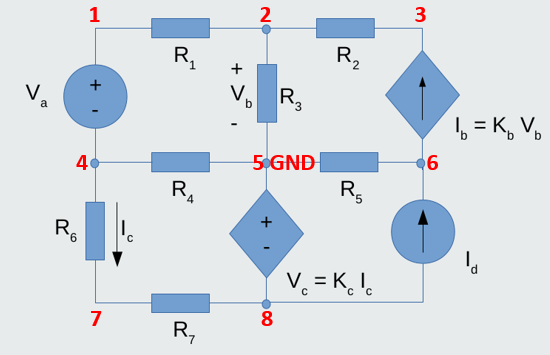
\includegraphics[width=0.8\linewidth]{Nodes.png}
    \centering
    \caption{Nodes Method applied to the circuit}
    \label{circuitlt}
\end{figure}


\par Then, the system of equations was written using the numeration stipulated above. There was a voltage source $V_T$ created to aid the analysis of the simulation.
$$
\begin{cases} 
	G_1(V_1-V_2)+G_2(V_3-V_2)-G_3V_b = 0 \\
	G_2(V_2-V_3)+V_b = 0 \\ 
	G_5(V_5-V_6)-V_b = -I_d \\
	G_6(V_4-V_7)-\frac{V_c}{K_c} = 0 \\
	G_7/(V_8-V_7)+\frac{V_c}{K_c} = 0 \\
	V_1-V_4 = V_a \\
	V_2-V_5-V_b = 0 \\
	V_5 = 0 \\
	V_5-V_8-V_c = 0 \\
	G_1(V_2-V_1)+G_4(V_5-V_4)-\frac{V_c}{K_c} = 0 
\label{system nodes}
\end{cases}
$$
\par The system above was then converted into a matrix equation \ref{matrixn} in order to have it solved by \textit{Octave}.
\begin{equation}
	\begin{bmatrix}
		G_1 & -G_1-G_2 & 0 & 0 & 0 & 0 & 0 & 0 & -G_3 & 0\\
		0 & G_2 & -G_2 & 0 & 0 & 0 & 0 & 0 & K_b & 0\\
		0 & 0 & 0 & 0 & G_5 & -G5 & 0 & 0 & -K_b & 0 \\
		0 & 0 & 0 & G_6 & 0 & 0 & -G_6 & 0 & 0 & -\frac{1}{K_c} \\
		0 & 0 & 0 & 0 & 0 & 0 & -G_7 & G_7 & 0 & \frac{1}{K_c} \\
		1 & 0 & 0 & -1 & 0 & 0 & 0 & 0 & 0 & 0\\
		0 & 1 & 0 & 0 & -1 & 0 & 0 & 0 & -1 & 0\\
		0 & 0 & 0 & 0 & 1 & 0 & 0 & 0 & 0 & 0\\
		0 & 0 & 0 & 0 & 1 & 0 & 0 & -1 & 0 & -1\\
		-G_1 & G_1 & 0 & -G_4 & G_4 & 0 & 0 & 0 & 0 & -\frac{1}{K_c} \\
	\end{bmatrix}
	\begin{bmatrix}
		V_1     \\
		V_2     \\
		V_3  \\
		V_4  \\
		V_5  \\
		V_6   \\
		V_7   \\ 
		V_8     \\
		V_b     \\
		V_c       \\
	\end{bmatrix}
    =
	\begin{bmatrix}
		0     \\
		0     \\
		-I_d  \\
		0     \\
		0     \\
		V_a     \\
		0     \\
		0     \\
		0     \\
		0     \\
	\end{bmatrix}
	\label{matrixn}
\end{equation}

\par With that, the values for $V_1$ up to $V_8$, $V_b$ and $V_c$ were achieved with the values afterwards displayed. The units for current and voltage are the same as in the mesh method.

\begin{table}[H]
  \centering
  \begin{tabular}{|c|c|}
    \hline    
    {\bf Name} & {\bf Value [V]} \\ \hline
    $V_5$ & 0.000000e+00 \\ \hline 
$V_1$ & 1.921818e-01 \\ \hline 
$V_2$ & -3.268625e-02 \\ \hline 
$V_3$ & -5.163789e-01 \\ \hline 
$V_4$ & -4.809026e+00 \\ \hline 
$V_6$ & 3.899261e+00 \\ \hline 
$V_7$ & -6.662760e+00 \\ \hline 
$V_8$ & -7.630992e+00 \\ \hline 
$V_a$ & 5.001208e+00 \\ \hline 
$V_b$ & -3.268625e-02 \\ \hline 
$V_c$ & 7.630992e+00 \\ \hline 

  \end{tabular}
  \caption{Nodes method results.}
  \label{tab:op}
\end{table}

\par It is now possible, with
\begin{equation}
	V_b=\frac{I_b}{K_b}
\label{Vb}
\end{equation}
and
\begin{equation}
	V_c=K_{c}I_{c}
\end{equation}
to obtain the values for all the voltages named in the circuit, $V_a$, $V_b$ and $V_c$:


\par It is visible that the values obtain in both methods present virtually identical values.

\par In the next section, these methods will be compared with a simulation of the circuit, with the aim of testing this theoretical analysis and discussing its results.
\newpage


\section{Simulation Analysis}
\label{sec:simulation}
\paragraph{}

\par This simulation was run through a software called NGSpice. From it, the results obtained were the following. 
\begin{table}[H]
  \centering
  \begin{tabular}{|c|c|}
    \hline    
    {\bf Name} & {\bf Value [A or V]} \\ \hline
    @g1[i] & -2.32920e-04\\ \hline
@i1[current] & 1.031362e-03\\ \hline
@r1[i] & -2.22464e-04\\ \hline
@r2[i] & -2.32920e-04\\ \hline
@r3[i] & -1.04564e-05\\ \hline
@r4[i] & 1.148500e-03\\ \hline
@r5[i] & 1.264282e-03\\ \hline
@r6[i] & -9.26037e-04\\ \hline
@r7[i] & -9.26037e-04\\ \hline
v0 & -4.80903e+00\\ \hline
v1 & 1.921818e-01\\ \hline
v2 & -3.26862e-02\\ \hline
v3 & -5.16379e-01\\ \hline
v4 & -4.80903e+00\\ \hline
v6 & 3.899261e+00\\ \hline
v7 & -6.66276e+00\\ \hline
v8 & -7.63099e+00\\ \hline

  \end{tabular}
  \caption{Operating point. A variable preceded by @ is of type {\em current}
    and expressed in Ampere; other variables are of type {\it voltage} and expressed in
    Volt.}
  \label{tab:op}
\end{table}

\par Such results are sufficient for a thourough analysis of the entire circuit. 
\par Firstly, by noting that $V_b$ is the imposed voltage between nodes 2 and 5, one concludes that $V_b$ is then given by $V_2$ given that node 5 is attached to ground. Likewise, and given that $V_c$ is the imposed voltage between nodes 5 and 8 and since node 5 is connected to ground, $V_c$ is then given by negative $V_8$.

\begin{equation}
	V_b=V_{2}
\end{equation}
\begin{equation}
	V_c=-V_{8}
\end{equation}

\par Secondly, by noting that currents passing through $R_1$, $R_2$ and $R_6$ are equal to $I_a$, $I_b$ and $I_c$ respectively, one can directly apply Ohms Law to determine these currents. While $I_b$ and $I_c$ could be determined through direct application of the law, it could also be determined by using the relation described in equations 3 and 4. 
\par From such calculations, the following results were obtained. 
\begin{table}[H]
    \centering
    \begin{tabular}{|c|c|}
    \hline
        $I_a$ & 2.40136e-04\\ \hline
        $I_b$ & 2.51245e-04\\ \hline
        $I_c$ & 9.76838e-04\\ \hline
        $V_b$ & 3.4437e-02\\ \hline
        $V_c$ & 7.979210e+00\\ \hline
    \end{tabular}
    \caption{Table of results for the simulation in A and V}
\end{table}





\section{Conclusion}
\label{sec:conclusion}
\paragraph{}
\par In this cirtcuit in specific there were only linear components, which enabled us to use the Kirchoff laws and subsequently the mesh and nodal analysis. Another consequence of this linearity is the superposition theroem, which is the basis for the mesh method, given it validates the concept of having more than one current going through a component, which can be viewed independently and allow for a method to succesfully discover all the unkowns in the circuit.
\par The nodal analysis is, as previously mentioned, the one that is easier to automize and is therefore included in \textit{NGSpice}, the simulator used in this activity. It was, therefore, possible to draw conclusions that validate this method that allows for the proper examination of the board.
\par It is now possible to affirm that both theoretical methods are viable due to the fact that similar results were obtained when calculated by a simulator. The previously mentioned linearity of the system accompanied by the success of the \textit{NGSpice} simulation prove this thesis.
\par Concluding, it is possible to analyze this circuit not only through simulation, but also theoretically using the Kirchoff Laws and the nodal and mesh methods because of circuits linearity.

%\cleardoublepage

% ----------------------------------------------------------------------
%  Bibliography
% ----------------------------------------------------------------------
%\addcontentsline{toc}{section}{\bibname}
%\bibliographystyle{abbrvunsrtnat} % <<<<< SELECT IF USING REFERENCES BY NUMBER (CITATION ORDER)
%\bibliography{../../../BIBfile.bib}

% ----------------------------------------------------------------------
\end{document}
% ----------------------------------------------------------------------
